% SOURCE: submissions/d2-neurocomputing/zenodo-deposit/results/merging/RG_map_evidence_REFIX20260801.json :: cells.*.per_g.{2,3,5,10,20}.{c2_coherent(>=2 seeds)+partial_rho_mean>=0.15 => qualifying g; saturated(<2 seeds) => gradated g; cells with no qualifying g marked with crosses, never dropped
% !TEX encoding = UTF-8 Unicode
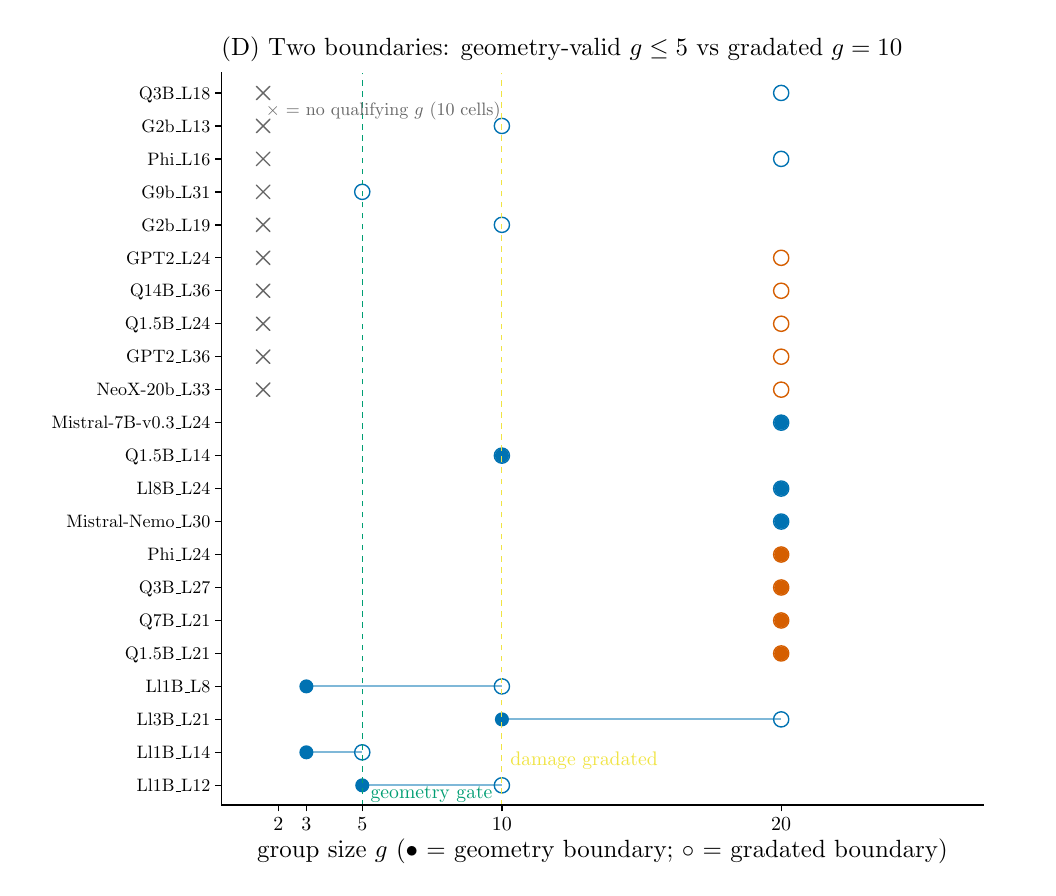
\begin{tikzpicture}[x=1pt,y=1pt]
\definecolor{fillColor}{RGB}{255,255,255}
\path[use as bounding box,fill=fillColor,fill opacity=0.00] (0,0) rectangle (361.35,303.53);
\begin{scope}
\path[clip] (  0.00,  0.00) rectangle (361.35,303.53);
\definecolor{drawColor}{RGB}{255,255,255}
\definecolor{fillColor}{RGB}{255,255,255}

\path[draw=drawColor,line width= 0.5pt,line join=round,line cap=round,fill=fillColor] (  0.00,  0.00) rectangle (361.35,303.53);
\end{scope}
\begin{scope}
\path[clip] ( 70.03, 22.61) rectangle (345.35,287.09);
\definecolor{fillColor}{RGB}{255,255,255}

\path[fill=fillColor] ( 70.03, 22.61) rectangle (345.35,287.09);
\definecolor{drawColor}{RGB}{0,114,178}

\path[draw=drawColor,draw opacity=0.50,line width= 0.7pt,line join=round] (100.71, 65.50) -- (171.36, 65.50);

\path[draw=drawColor,draw opacity=0.50,line width= 0.7pt,line join=round] (171.36, 53.58) -- (272.28, 53.58);

\path[draw=drawColor,draw opacity=0.50,line width= 0.7pt,line join=round] (100.71, 41.67) -- (120.90, 41.67);

\path[draw=drawColor,draw opacity=0.50,line width= 0.7pt,line join=round] (120.90, 29.75) -- (171.36, 29.75);
\definecolor{fillColor}{RGB}{0,114,178}

\path[fill=fillColor] (100.71, 65.50) circle (  2.54);

\path[fill=fillColor] (171.36, 53.58) circle (  2.54);

\path[fill=fillColor] (100.71, 41.67) circle (  2.54);

\path[fill=fillColor] (272.28,160.80) circle (  2.54);

\path[fill=fillColor] (171.36,148.89) circle (  2.54);

\path[fill=fillColor] (120.90, 29.75) circle (  2.54);

\path[fill=fillColor] (272.28,136.98) circle (  2.54);

\path[fill=fillColor] (272.28,125.06) circle (  2.54);
\definecolor{fillColor}{RGB}{213,94,0}

\path[fill=fillColor] (272.28,113.15) circle (  2.54);

\path[fill=fillColor] (272.28,101.24) circle (  2.54);

\path[fill=fillColor] (272.28, 89.32) circle (  2.54);

\path[fill=fillColor] (272.28, 77.41) circle (  2.54);
\definecolor{drawColor}{RGB}{0,114,178}

\path[draw=drawColor,line width= 0.5pt,line join=round,line cap=round] (171.36, 65.50) circle (  2.75);

\path[draw=drawColor,line width= 0.5pt,line join=round,line cap=round] (272.28,279.94) circle (  2.75);

\path[draw=drawColor,line width= 0.5pt,line join=round,line cap=round] (272.28, 53.58) circle (  2.75);

\path[draw=drawColor,line width= 0.5pt,line join=round,line cap=round] (120.90, 41.67) circle (  2.75);

\path[draw=drawColor,line width= 0.5pt,line join=round,line cap=round] (272.28,160.80) circle (  2.75);

\path[draw=drawColor,line width= 0.5pt,line join=round,line cap=round] (171.36,148.89) circle (  2.75);

\path[draw=drawColor,line width= 0.5pt,line join=round,line cap=round] (171.36, 29.75) circle (  2.75);

\path[draw=drawColor,line width= 0.5pt,line join=round,line cap=round] (272.28,136.98) circle (  2.75);

\path[draw=drawColor,line width= 0.5pt,line join=round,line cap=round] (171.36,268.02) circle (  2.75);

\path[draw=drawColor,line width= 0.5pt,line join=round,line cap=round] (272.28,256.11) circle (  2.75);

\path[draw=drawColor,line width= 0.5pt,line join=round,line cap=round] (120.90,244.20) circle (  2.75);

\path[draw=drawColor,line width= 0.5pt,line join=round,line cap=round] (171.36,232.28) circle (  2.75);

\path[draw=drawColor,line width= 0.5pt,line join=round,line cap=round] (272.28,125.06) circle (  2.75);
\definecolor{drawColor}{RGB}{213,94,0}

\path[draw=drawColor,line width= 0.5pt,line join=round,line cap=round] (272.28,113.15) circle (  2.75);

\path[draw=drawColor,line width= 0.5pt,line join=round,line cap=round] (272.28,101.24) circle (  2.75);

\path[draw=drawColor,line width= 0.5pt,line join=round,line cap=round] (272.28, 89.32) circle (  2.75);

\path[draw=drawColor,line width= 0.5pt,line join=round,line cap=round] (272.28,220.37) circle (  2.75);

\path[draw=drawColor,line width= 0.5pt,line join=round,line cap=round] (272.28, 77.41) circle (  2.75);

\path[draw=drawColor,line width= 0.5pt,line join=round,line cap=round] (272.28,208.46) circle (  2.75);

\path[draw=drawColor,line width= 0.5pt,line join=round,line cap=round] (272.28,196.54) circle (  2.75);

\path[draw=drawColor,line width= 0.5pt,line join=round,line cap=round] (272.28,184.63) circle (  2.75);

\path[draw=drawColor,line width= 0.5pt,line join=round,line cap=round] (272.28,172.72) circle (  2.75);
\definecolor{drawColor}{gray}{0.40}

\path[draw=drawColor,line width= 0.5pt,line join=round,line cap=round] ( 82.65,277.51) -- ( 87.50,282.36);

\path[draw=drawColor,line width= 0.5pt,line join=round,line cap=round] ( 82.65,282.36) -- ( 87.50,277.51);

\path[draw=drawColor,line width= 0.5pt,line join=round,line cap=round] ( 82.65,265.60) -- ( 87.50,270.45);

\path[draw=drawColor,line width= 0.5pt,line join=round,line cap=round] ( 82.65,270.45) -- ( 87.50,265.60);

\path[draw=drawColor,line width= 0.5pt,line join=round,line cap=round] ( 82.65,253.69) -- ( 87.50,258.54);

\path[draw=drawColor,line width= 0.5pt,line join=round,line cap=round] ( 82.65,258.54) -- ( 87.50,253.69);

\path[draw=drawColor,line width= 0.5pt,line join=round,line cap=round] ( 82.65,241.77) -- ( 87.50,246.62);

\path[draw=drawColor,line width= 0.5pt,line join=round,line cap=round] ( 82.65,246.62) -- ( 87.50,241.77);

\path[draw=drawColor,line width= 0.5pt,line join=round,line cap=round] ( 82.65,229.86) -- ( 87.50,234.71);

\path[draw=drawColor,line width= 0.5pt,line join=round,line cap=round] ( 82.65,234.71) -- ( 87.50,229.86);

\path[draw=drawColor,line width= 0.5pt,line join=round,line cap=round] ( 82.65,217.94) -- ( 87.50,222.80);

\path[draw=drawColor,line width= 0.5pt,line join=round,line cap=round] ( 82.65,222.80) -- ( 87.50,217.94);

\path[draw=drawColor,line width= 0.5pt,line join=round,line cap=round] ( 82.65,206.03) -- ( 87.50,210.88);

\path[draw=drawColor,line width= 0.5pt,line join=round,line cap=round] ( 82.65,210.88) -- ( 87.50,206.03);

\path[draw=drawColor,line width= 0.5pt,line join=round,line cap=round] ( 82.65,194.12) -- ( 87.50,198.97);

\path[draw=drawColor,line width= 0.5pt,line join=round,line cap=round] ( 82.65,198.97) -- ( 87.50,194.12);

\path[draw=drawColor,line width= 0.5pt,line join=round,line cap=round] ( 82.65,182.20) -- ( 87.50,187.06);

\path[draw=drawColor,line width= 0.5pt,line join=round,line cap=round] ( 82.65,187.06) -- ( 87.50,182.20);

\path[draw=drawColor,line width= 0.5pt,line join=round,line cap=round] ( 82.65,170.29) -- ( 87.50,175.14);

\path[draw=drawColor,line width= 0.5pt,line join=round,line cap=round] ( 82.65,175.14) -- ( 87.50,170.29);
\definecolor{drawColor}{RGB}{0,158,115}

\path[draw=drawColor,line width= 0.4pt,dash pattern=on 2pt off 2pt ,line join=round] (120.90, 22.61) -- (120.90,287.09);
\definecolor{drawColor}{RGB}{240,228,66}

\path[draw=drawColor,line width= 0.4pt,dash pattern=on 2pt off 2pt ,line join=round] (171.36, 22.61) -- (171.36,287.09);
\definecolor{drawColor}{RGB}{0,158,115}

\node[text=drawColor,anchor=base west,inner sep=0pt, outer sep=0pt, scale=  0.71] at (123.93, 24.92) {geometry gate};
\definecolor{drawColor}{RGB}{240,228,66}

\node[text=drawColor,anchor=base west,inner sep=0pt, outer sep=0pt, scale=  0.71] at (174.39, 36.84) {damage gradated};
\definecolor{drawColor}{gray}{0.40}

\node[text=drawColor,anchor=base west,inner sep=0pt, outer sep=0pt, scale=  0.65] at ( 86.08,271.73) {$\times$ = no qualifying $g$ (10 cells)};
\end{scope}
\begin{scope}
\path[clip] (  0.00,  0.00) rectangle (361.35,303.53);
\definecolor{drawColor}{RGB}{0,0,0}

\path[draw=drawColor,line width= 0.5pt,line join=round,line cap=rect] ( 70.03, 22.61) --
	( 70.03,287.09);
\end{scope}
\begin{scope}
\path[clip] (  0.00,  0.00) rectangle (361.35,303.53);
\definecolor{drawColor}{RGB}{0,0,0}

\node[text=drawColor,anchor=base east,inner sep=0pt, outer sep=0pt, scale=  0.65] at ( 65.98, 27.52) {Ll1B\_L12};

\node[text=drawColor,anchor=base east,inner sep=0pt, outer sep=0pt, scale=  0.65] at ( 65.98, 39.43) {Ll1B\_L14};

\node[text=drawColor,anchor=base east,inner sep=0pt, outer sep=0pt, scale=  0.65] at ( 65.98, 51.34) {Ll3B\_L21};

\node[text=drawColor,anchor=base east,inner sep=0pt, outer sep=0pt, scale=  0.65] at ( 65.98, 63.26) {Ll1B\_L8};

\node[text=drawColor,anchor=base east,inner sep=0pt, outer sep=0pt, scale=  0.65] at ( 65.98, 75.17) {Q1.5B\_L21};

\node[text=drawColor,anchor=base east,inner sep=0pt, outer sep=0pt, scale=  0.65] at ( 65.98, 87.08) {Q7B\_L21};

\node[text=drawColor,anchor=base east,inner sep=0pt, outer sep=0pt, scale=  0.65] at ( 65.98, 99.00) {Q3B\_L27};

\node[text=drawColor,anchor=base east,inner sep=0pt, outer sep=0pt, scale=  0.65] at ( 65.98,110.91) {Phi\_L24};

\node[text=drawColor,anchor=base east,inner sep=0pt, outer sep=0pt, scale=  0.65] at ( 65.98,122.82) {Mistral-Nemo\_L30};

\node[text=drawColor,anchor=base east,inner sep=0pt, outer sep=0pt, scale=  0.65] at ( 65.98,134.74) {Ll8B\_L24};

\node[text=drawColor,anchor=base east,inner sep=0pt, outer sep=0pt, scale=  0.65] at ( 65.98,146.65) {Q1.5B\_L14};

\node[text=drawColor,anchor=base east,inner sep=0pt, outer sep=0pt, scale=  0.65] at ( 65.98,158.56) {Mistral-7B-v0.3\_L24};

\node[text=drawColor,anchor=base east,inner sep=0pt, outer sep=0pt, scale=  0.65] at ( 65.98,170.48) {NeoX-20b\_L33};

\node[text=drawColor,anchor=base east,inner sep=0pt, outer sep=0pt, scale=  0.65] at ( 65.98,182.39) {GPT2\_L36};

\node[text=drawColor,anchor=base east,inner sep=0pt, outer sep=0pt, scale=  0.65] at ( 65.98,194.31) {Q1.5B\_L24};

\node[text=drawColor,anchor=base east,inner sep=0pt, outer sep=0pt, scale=  0.65] at ( 65.98,206.22) {Q14B\_L36};

\node[text=drawColor,anchor=base east,inner sep=0pt, outer sep=0pt, scale=  0.65] at ( 65.98,218.13) {GPT2\_L24};

\node[text=drawColor,anchor=base east,inner sep=0pt, outer sep=0pt, scale=  0.65] at ( 65.98,230.05) {G2b\_L19};

\node[text=drawColor,anchor=base east,inner sep=0pt, outer sep=0pt, scale=  0.65] at ( 65.98,241.96) {G9b\_L31};

\node[text=drawColor,anchor=base east,inner sep=0pt, outer sep=0pt, scale=  0.65] at ( 65.98,253.87) {Phi\_L16};

\node[text=drawColor,anchor=base east,inner sep=0pt, outer sep=0pt, scale=  0.65] at ( 65.98,265.79) {G2b\_L13};

\node[text=drawColor,anchor=base east,inner sep=0pt, outer sep=0pt, scale=  0.65] at ( 65.98,277.70) {Q3B\_L18};
\end{scope}
\begin{scope}
\path[clip] (  0.00,  0.00) rectangle (361.35,303.53);
\definecolor{drawColor}{RGB}{0,0,0}

\path[draw=drawColor,line width= 0.5pt,line join=round] ( 67.78, 29.75) --
	( 70.03, 29.75);

\path[draw=drawColor,line width= 0.5pt,line join=round] ( 67.78, 41.67) --
	( 70.03, 41.67);

\path[draw=drawColor,line width= 0.5pt,line join=round] ( 67.78, 53.58) --
	( 70.03, 53.58);

\path[draw=drawColor,line width= 0.5pt,line join=round] ( 67.78, 65.50) --
	( 70.03, 65.50);

\path[draw=drawColor,line width= 0.5pt,line join=round] ( 67.78, 77.41) --
	( 70.03, 77.41);

\path[draw=drawColor,line width= 0.5pt,line join=round] ( 67.78, 89.32) --
	( 70.03, 89.32);

\path[draw=drawColor,line width= 0.5pt,line join=round] ( 67.78,101.24) --
	( 70.03,101.24);

\path[draw=drawColor,line width= 0.5pt,line join=round] ( 67.78,113.15) --
	( 70.03,113.15);

\path[draw=drawColor,line width= 0.5pt,line join=round] ( 67.78,125.06) --
	( 70.03,125.06);

\path[draw=drawColor,line width= 0.5pt,line join=round] ( 67.78,136.98) --
	( 70.03,136.98);

\path[draw=drawColor,line width= 0.5pt,line join=round] ( 67.78,148.89) --
	( 70.03,148.89);

\path[draw=drawColor,line width= 0.5pt,line join=round] ( 67.78,160.80) --
	( 70.03,160.80);

\path[draw=drawColor,line width= 0.5pt,line join=round] ( 67.78,172.72) --
	( 70.03,172.72);

\path[draw=drawColor,line width= 0.5pt,line join=round] ( 67.78,184.63) --
	( 70.03,184.63);

\path[draw=drawColor,line width= 0.5pt,line join=round] ( 67.78,196.54) --
	( 70.03,196.54);

\path[draw=drawColor,line width= 0.5pt,line join=round] ( 67.78,208.46) --
	( 70.03,208.46);

\path[draw=drawColor,line width= 0.5pt,line join=round] ( 67.78,220.37) --
	( 70.03,220.37);

\path[draw=drawColor,line width= 0.5pt,line join=round] ( 67.78,232.28) --
	( 70.03,232.28);

\path[draw=drawColor,line width= 0.5pt,line join=round] ( 67.78,244.20) --
	( 70.03,244.20);

\path[draw=drawColor,line width= 0.5pt,line join=round] ( 67.78,256.11) --
	( 70.03,256.11);

\path[draw=drawColor,line width= 0.5pt,line join=round] ( 67.78,268.02) --
	( 70.03,268.02);

\path[draw=drawColor,line width= 0.5pt,line join=round] ( 67.78,279.94) --
	( 70.03,279.94);
\end{scope}
\begin{scope}
\path[clip] (  0.00,  0.00) rectangle (361.35,303.53);
\definecolor{drawColor}{RGB}{0,0,0}

\path[draw=drawColor,line width= 0.5pt,line join=round,line cap=rect] ( 70.03, 22.61) --
	(345.35, 22.61);
\end{scope}
\begin{scope}
\path[clip] (  0.00,  0.00) rectangle (361.35,303.53);
\definecolor{drawColor}{RGB}{0,0,0}

\path[draw=drawColor,line width= 0.5pt,line join=round] ( 90.62, 20.36) --
	( 90.62, 22.61);

\path[draw=drawColor,line width= 0.5pt,line join=round] (100.71, 20.36) --
	(100.71, 22.61);

\path[draw=drawColor,line width= 0.5pt,line join=round] (120.90, 20.36) --
	(120.90, 22.61);

\path[draw=drawColor,line width= 0.5pt,line join=round] (171.36, 20.36) --
	(171.36, 22.61);

\path[draw=drawColor,line width= 0.5pt,line join=round] (272.28, 20.36) --
	(272.28, 22.61);
\end{scope}
\begin{scope}
\path[clip] (  0.00,  0.00) rectangle (361.35,303.53);
\definecolor{drawColor}{RGB}{0,0,0}

\node[text=drawColor,anchor=base,inner sep=0pt, outer sep=0pt, scale=  0.72] at ( 90.62, 13.60) {2};

\node[text=drawColor,anchor=base,inner sep=0pt, outer sep=0pt, scale=  0.72] at (100.71, 13.60) {3};

\node[text=drawColor,anchor=base,inner sep=0pt, outer sep=0pt, scale=  0.72] at (120.90, 13.60) {5};

\node[text=drawColor,anchor=base,inner sep=0pt, outer sep=0pt, scale=  0.72] at (171.36, 13.60) {10};

\node[text=drawColor,anchor=base,inner sep=0pt, outer sep=0pt, scale=  0.72] at (272.28, 13.60) {20};
\end{scope}
\begin{scope}
\path[clip] (  0.00,  0.00) rectangle (361.35,303.53);
\definecolor{drawColor}{RGB}{0,0,0}

\node[text=drawColor,anchor=base,inner sep=0pt, outer sep=0pt, scale=  0.90] at (207.69,  3.75) {group size $g$ ($\bullet$ = geometry boundary; $\circ$ = gradated boundary)};
\end{scope}
\begin{scope}
\path[clip] (  0.00,  0.00) rectangle (361.35,303.53);
\definecolor{drawColor}{RGB}{0,0,0}

\node[text=drawColor,anchor=base west,inner sep=0pt, outer sep=0pt, scale=  0.90] at ( 70.03,293.34) {(D) Two boundaries: geometry-valid $g\leq5$ vs gradated $g=10$};
\end{scope}
\end{tikzpicture}
